% EdDSA for Baby Jubjub Elliptic Curve with MiMC-7 Hash.

\documentclass{article}
\usepackage[english]{babel}
\usepackage[utf8]{inputenc}
\usepackage{amsmath, amsthm, amssymb}
\usepackage{enumerate, enumitem}
\usepackage{graphicx}
\usepackage{color, xcolor}
\usepackage{setspace}
\usepackage{hyperref}
\usepackage{authblk}
\usepackage{tikz}
\usetikzlibrary{arrows}
\usetikzlibrary{positioning}
\usepackage{mathtools}
%floor vs. ceil
\DeclarePairedDelimiter{\floor}{\lfloor}{\rfloor} 
\DeclarePairedDelimiter{\ceil}{\lceil}{\rceil}  % If called \ceil*{x} it will add left/right.

%\usepackage{algorithmicx}
\usepackage{algorithm}
\usepackage[noend]{algpseudocode}
\makeatletter
\def\BState{\State\hskip-\ALG@thistlm}
\makeatother
%\usepackage{listings}
%\lstdefinelanguage{Sage}[]{Python}
%{morekeywords={False,sage,True},sensitive=true}
%\lstset{
%  frame=none,
%  showtabs=False,
%  showspaces=False,
%  showstringspaces=False,
%  commentstyle={\ttfamily\color{dgreencolor}},
%  keywordstyle={\ttfamily\color{dbluecolor}\bfseries},
%  stringstyle={\ttfamily\color{dgraycolor}\bfseries},
%  language=Sage,
%  basicstyle={\fontsize{10pt}{10pt}\ttfamily},
%  aboveskip=0.3em,
%  belowskip=0.1em,
%  numbers=left,
%  numberstyle=\footnotesize
%}


\textwidth 16 cm
\textheight 22 cm
\topmargin -1 cm
\oddsidemargin -0 cm

\addtolength{\skip\footins}{1pc plus 5pt} % Foot note space
\setlength\parindent{0pt} % No indent

\newcommand{\N}{\ensuremath{\mathbb{N}}}
\newcommand{\Np}{\ensuremath{\mathbb{N}^{+}}}
\newcommand{\Z}{\ensuremath{\mathbb{Z}}}
\newcommand{\Q}{\ensuremath{\mathbb{Q}}}
\newcommand{\R}{\ensuremath{\mathbb{R}}}
\newcommand{\C}{\ensuremath{\mathbb{C}}}
\newcommand{\Fp}{\ensuremath{\mathbb{F}_p}}
\newcommand{\Fr}{\ensuremath{\mathbb{F}_r}}
\newcommand{\G}{\ensuremath{\mathbb{G}}}
\newcommand{\point}[1]{P_{#1} = (x_{#1}, y_{#1})}
\newcommand{\llog}{\log_2}
\newcommand{\xor}{\oplus}
\newcommand{\minSize}{1.5em}
\newcommand{\gen}[1]{\ensuremath{\langle #1\rangle}}
\newcommand{\noi}{\noindent}

\tikzset{%
	leaf/.style = {draw, fill}, %, minimum size=\minSize},
	empty/.style = {draw},
	wrong/.style = {draw, fill = red},
	internal/.style = {draw, path picture={\draw 
			(path picture bounding box.south east) -- (path picture bounding box.north west) 		(path picture bounding box.south west) -- (path picture bounding box.north east);}}
}

\makeatletter
\renewcommand\AB@affilsepx{, \protect\Affilfont}
\makeatother

\title{ EdDSA for Baby Jubjub Elliptic Curve with MiMC-7 Hash \vspace{-0.2cm} }
\author[1]{Jordi Baylina}
\author[1,2]{Marta Bellés}
\affil[1]{iden3}
\affil[2]{Universitat Pompeu Fabra}
\date{}
\setcounter{Maxaffil}{0}
\renewcommand\Affilfont{\itshape\small}


\begin{document}
\begin{spacing}{1.2}
\maketitle 
\vspace{1cm}
\tableofcontents
		
\vspace{0.5cm}
		
\newpage
		
\section{Scope}

This proposal aims to standardize the elliptic curve signature scheme Edwards-curve Digital Signature Algorithm (EdDSA) for Baby Jubjub Edwards elliptic curve using MiMC-7 hash function.
		
\section{Motivation}

EdDSA is a variant of Schnorr's signature scheme and it provides high performance on a variety of platforms \cite{eddsa}. 
		
\section{Background}

There are many implementations of EdDSA with Edwards elliptic curves such as Ed25519 or Ed448-Goldilocks and most of them use hash SHA-512. This is the first document specifying a protocol for implementing EdDSA using MiMC-7 and we describe it on the Baby Jubjub Elliptic curve.  \\
		
The choice of the MiMC-7 hash function makes computations inside circuits very efficient and it has a big potential in zero knowledge protocols such as zk-SNARK.

\section{Terminology}

The table below summarizes the terminology used across the document. Each element is explained in greater detail in the following sections.

	\begin{table}[h!]
	\centering
	\begin{tabular}{|l|l|}
		\hline
		{\bf Notation} & {\bf Description}\\
		\hline
		{$p$} & {Prime number.}\\
		{$\Fp$} & {Finite field with $p$ elements.}\\
		{$E$} & {Baby Jubjub elliptic curve (defined over $Fp$) in Edwards form.}\\
		{$E_M$} & {Baby Jubjub elliptic curve (defined over $Fp$) in Montgomery form.}\\
		{$l$} & {Large prime number dividing the order of Baby Jubjub.}\\
		{$\Fl$} & {Finite field with $l$ elements.}\\
		{$\G$} & {Group of $\Fp$-rational points of order $l$.}\\
		{$B$} & {Base point (generator of $\G$) of Baby Jubjub.}\\
		\hline
		{$A = (A_x, A_y)$} & {Public key. $A$ is a point on $E$. }\\
		$k$ & Private key. \\
		$M$ & Message. $M$ is an element of $\Fl$. \\		
		{$(R,S) = ((R_x, R_y), S)$} & Signature on $M$. $R$ is a point on $E$ and $S$ and element of $\Fl$.\\
		\hline		
		{$H$} & {Hash function MiMC-7.}\\
		$r$ & Number of rounds of MiMC-7. \\
		$c_0, c_1, \dots, c_r$ & Constants used in MiMC-7. \\
		\hline
	\end{tabular}
	\label{tab:notation}
	\end{table}

	\subsection{Baby-Jubjub} 	%Consider the prime number 
$$	p = 21888242871839275222246405745257275088548364
400416034343698204186575808495617 $$
and let $\Fp$ be the finite field with $p$ elements. 

% \subsubsection{Montgomery form}
%{\it{Baby-Jubjub}} is birationally equivalent to the Montgomery elliptic curve defined by  
	$$ E_M : v^2 = u^3 + 168698 u^2 + u. $$
The birational equivalence from $E$ to $E_M$ is the map 
	$$ (x,y) \to (u,v) = \left( \frac{1 + y}{1 - y} , \frac{1 + y}{(1 - y)x} \right) $$
with inverse from $E_M$ to $E$
	$$ (u, v) \to (x, y) = \left(  \frac{u}{v}, \frac{u - 1}{u + 1}   \right). $$
These results are from \cite[Theorem 3.2]{twisted}.
We define $E_M$ as the {\it Baby-Jubjub} Montgomery elliptic curve defined over $\Fp$ given %described
by equation
$$	E: v^2 = u^3 +  168698u^2 + u. $$
The order of $E_M$ is $n = 8\times r$, where 
$$	r = 2736030358979909402780800718157159386076813972
158567259200215660948447373041 $$ 
is a prime number. Denote by $\G$ the subgroup of points of order $r$, that is, %of $E$ 
$$\G = \Set{ P \in E(\Fp) | r P = O  }.$$

% \subsubsection{Edwards form}
$E_M$ is birationally equivalent to the Edwards elliptic curve %[REF] defined by  
$$	E: x^2 + y^2 = 1 +  d x^2 y^2 $$
where
$ d = 9706598848417545097372247223557719406784115219466060233080913168975159366771.$ \\

% \subsubsection{Birational equivalence}

The birational equivalence \cite[Thm. 3.2]{twisted} from $E$ to $E_M$ is the map
% These results are from \cite[Theorem 3.2]{twisted}. 
$$ (x,y) \to (u,v) = \left( \frac{1 + y}{1 - y} , \frac{1 + y}{(1 - y)x} \right) $$
with inverse from $E_M$ to $E$
$$ (u, v) \to (x, y) = \left(  \frac{u}{v}, \frac{u - 1}{u + 1}   \right). $$

	
	Consider the prime number 
		$$	p = 21888242871839275222246405745257275088548364400416034343698204186575808495617 $$
	and let $\Fp$ be the finite field with $p$ elements. We define $E_M$ as the {\it Baby-Jubjub} Montgomery elliptic curve defined over $\Fp$ given by equation
		$$	E: v^2 = u^3 +  168698u^2 + u. $$
	The order of $E_M$ is $n = 8\times l$, where 
		$$	l = 2736030358979909402780800718157159386076813972158567259200215660948447373041 $$ 
	is a prime number. Denote by $\G$ the subgroup of points of order $l$, that is, %of $E$ 
		$$\G = \Set{ P \in E(\Fp) | l P = O  }.$$
	Let
		\begin{align*} 
		B =  (17777552123799933955779906779655732241715742912184938656739573121738514868268,\\
		2626589144620713026669568689430873010625803728049924121243784502389097019475)
		\end{align*}
	be a generator of $\G$.\\
	
	$E_M$ is birationally equivalent to the Edwards elliptic curve %[REF] defined by  
		$$	E: x^2 + y^2 = 1 +  d x^2 y^2 $$
	where
		$ d = 9706598848417545097372247223557719406784115219466060233080913168975159366771.$ \\
	
	The birational equivalence \cite[Thm. 3.2]{twisted} from $E$ to $E_M$ is the map 
		$$ (x,y) \to (u,v) = \left( \frac{1 + y}{1 - y} , \frac{1 + y}{(1 - y)x} \right) $$
	with inverse from $E_M$ to $E$
		$$ (u, v) \to (x, y) = \left(  \frac{u}{v}, \frac{u - 1}{u + 1}   \right). $$
	
	\subsection{MiMC-7}
	
	The hash function used in EdDSA is MiMC-7 based in paper \cite{mimc}, which describes the hash using exponent 3. In this specification, we use exponent 7 (hence the name MiMC-7) as 3 and $l-1$ are not coprime and 7 is the optimal choice for exponentiation \cite[Sec. 6]{mimc}.\\
	
	Let $\Fl$ be the finite field with $l$ elements. The block cipher is constructed by iterating a round function $r$ times where each round consists of a key addition with the key $k$, the addition of a round constant $c_i\in \Fr$, and the application of a non-linear function defined as $F(x) :=x^7$ for $x\in \Fl$. The ciphertext is finally produced by adding the key $k$ again to the output of the last round. Hence, the round function is described as $F_i(x) = F(x) \xor k \xor c_i$ where $c_0 = c_r = 0$ and the encryption process is defined as 
		$$ E_k(x) = (F_{r-1} \circ F_{r-2} \circ ... \circ F_0)(x) \xor k. $$
		
	% !TEX root =/Users/martabellesmunoz/Dropbox/Documents/Especificacions/Merkle trees/Description.tex

\tikzstyle{exp} = [draw, minimum size=2em] % fill=blue!20,
\tikzstyle{init} = [pin edge={to-,thin,black}]
\tikzset{XOR/.style={draw,circle,append after command={
        [shorten >=\pgflinewidth, shorten <=\pgflinewidth,]
        (\tikzlastnode.north) edge (\tikzlastnode.south)
        (\tikzlastnode.east) edge (\tikzlastnode.west)
        }}
}

\begin{center}
\begin{tikzpicture}[node distance=1.5cm, auto,>=latex']

    \node  (in) {$x$};
    \node [XOR, pin={[init]above:$k$}] (xor0) [right of=in, node distance=1cm]  { };
    \node [exp] (e0) [right of=xor0] {$x^7$};
    \node [XOR, pin={[init]above:$k \oplus c_1 $}] (xor1) [right of=e0] { };
    \node [exp] (e1) [right of=xor1] {$x^7$};
    \node [XOR, pin={[init]above:$k \oplus c_{r-1} $}] (xorr-1) [right of=e1, node distance=4cm] { };
    \node [exp] (er-1) [right of=xorr-1] {$x^7$};
    \node [XOR, pin={[init]above:$k \oplus c_r $}] (xor)  [right of=er-1] { };
    \node  (out)  [right of=xor, node distance=1cm] {$y$};

    \path[->] (in) edge node { } (xor0);
    \path[->] (xor0) edge node { } (e0);
    \path[->] (e0) edge node { } (xor1);
    \path[->] (xor1) edge node { } (e1);
    \path[->] (e1) edge[dotted] node { } (xorr-1);
    \path[->] (xorr-1) edge node {} (er-1);
    \path[->] (er-1) edge node { } (xor);
    \path[->] (xor) edge node { } (out);
   
\end{tikzpicture}
\end{center}

	
	As the random  constants $c_i$ do  not  need  to  be  generated  for  every evaluation of MiMC-7, they are hard-coded into the implementation. The generation of these constants and the required number of rounds is described in section \ref{sec-mimc}. 
	
	\subsection{EdDSA}
		
	The description of this protocol is based in \cite{eddsa}:  	
	Let the public key be a point $A = (A_x, A_y)\in E$ of order $l$ and $M$ a message we wish to sign. The signature on $M$ by $A$ consists of a par $(R,S)$ where $R = (R_x, R_y)$ is a point of order $l$ of $E$ and $S\in\Fl\backslash\{0\}$ such that 
	$$ 8SB = 8R + 8H(R,A,M)A.	$$
	
\section{Challenges and Security}

One of the main challenges to create this standard and to see it adopted by the community is to provide correct, usable, and well-maintained implementations in as many languages as possible. 
%
Some effort is also required to audit and verify code coming from the community and claiming
to implement EdDSA for Baby Jubjub to prevent the propagation of potentially
insecure implementations. Part of the work in progress of looking batch verification of short signatures. 
%
Lastly, the proposal as it stands uses MiMC-7 as hash function as it works very optimal inside circuits. We believe some work is required to determinate the security MiMC hash functions. 
	
\section{Implementation}

In this section, we specify how each of the main operations in the following EdDSA circuit are computed:

	\begin{figure}[h]
		\centering
		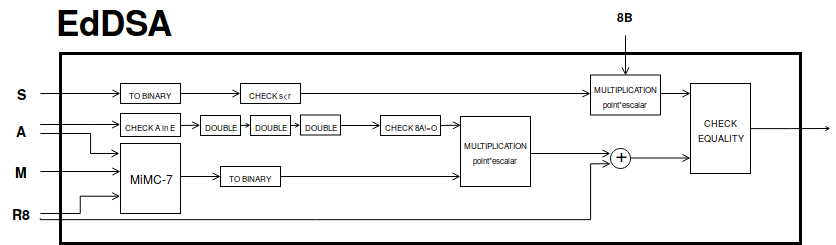
\includegraphics[scale=0.4]{../../figures/circuit-eddsa.png}
	\end{figure}

	\subsection{Operations in the Elliptic Curve}
		\subsubsection{Addition of Points}

		When adding points of elliptic curves in Montgomery form, one has to be careful if the points being added are equal (doubling) or not (adding) and if one of the points is the point at infinity \cite{montgomery}. 
		%
		Edwards curves have the advantage that there is no such case distinction and doubling can be performed with exactly the same formula as addition \cite{twisted}. 
		%
		In comparison, operating in Montgomery curves is cheaper. In this section, we summarize how addition and doubling is performed in both forms. 
		%
		For the exact number of operations required in different forms of elliptic curves, see \cite{twisted}.
		
		\begin{itemize}
			
			\item \underline{Edwards}: 	
			Let $\point{1}$ and $\point{2}$ be points of the Baby-Jubjub twisted Edwards elliptic curve $E$. The sum $P_1 + P_2$ is a third point $P_3 = (x_3, y_3)$ with 
				\begin{align*}
				&\lambda = d x_1x_2y_1y_2,\\
				&x_3 = (x_1y_2 + y_1x_2) / (1 + \lambda),\\
				&y_3 = (y_1y_2 - x_1x_2) / (1 - \lambda).
				\end{align*}
			Note that the neutral element is the point $O = (0,1)$ and the inverse of a point $(x,y)$ is $(-x,y)$.
			
			\item \underline{Montgomery}: 
			Let $\point{1}\not=O$ and $\point{2}\not=O$ be two points of the Baby-JubJub elliptic curve $E_M$ in Montgomery form. 
			
			If $P_1\not=P_2$, then the sum $P_1 + P_2$ is a third point $P_3 = (x_3, y_3)$ with coordinates
			\begin{align}
			\label{eq-ted}
				\begin{split}
				&\Lambda = (y_2-y_1)/ (x_2-x_1),\\
				&x_3 = \Lambda^2 - A - x_1 - x_2,\\
				&y_3 = \Lambda(x_1- x_3) - y_1.
				\end{split}
			\end{align}
			
			If $P_1 = P_2$, then $2\cdot P_1$ is a point $P_3 = (x_3, y_3)$ with coordinates
			\begin{align}
			\label{eq-mont}
				\begin{split}
				&\Lambda = (3x_1^2 + 2Ax_1 + 1)/ (2y_1),\\
				&x_3 = \Lambda^2 - A - 2x_1,\\
				&y_3 = \Lambda(x_1- x_3) - y_1.
				\end{split}	
			\end{align}
			
		\end{itemize}
	
	
		\subsubsection{Multiplication of a Point of $E$ by a Scalar}
		
		Let $P\not= O$ be a point of the Edwards curve $E$ of order strictly greater than 8 (i.e. $P\in\G$) and let $k$ a binary number representing an element of $\Fp$. We describe the circuit used to compute the point $k\cdot P$.
		
		\begin{enumerate}
			
			\item First, we divide $k$ into chunks of 248 bits. If $k$ is not a multiple of 248, we take $j$ segments of 248 bits and leave a last chunk with the remaining bits. More precisly, write 
			% TODO: The reason we do this? Dir que $r$ són tants bits (248)?
			\begin{gather*}
			k = k_0 k_1 \dots k_j 	\quad\text{with}\quad 
				\begin{cases}
				k_i = b^i_0 b^i_1 \dots b^i_{247} 	\;\text{ for }  i = 0, \dots, j-1, \\
				k_j = b^j_0 b^j_1 \dots b^j_s 	\;\text{ with } s\leq 247.
				\end{cases}
			\end{gather*}
			Then,  
			\begin{equation}
			\label{kP}
			k\cdot P = k_0\cdot P + k_1\cdot 2^{248}P +\dots+ k_j\cdot 2^{248j}P. 	
			\end{equation}
			This sum is done using the following circuit. 
			The terms of the sum are calculated separately inside the \textsc{seq} boxes and then added together. 
			
			\begin{figure}[h]
				\centering
				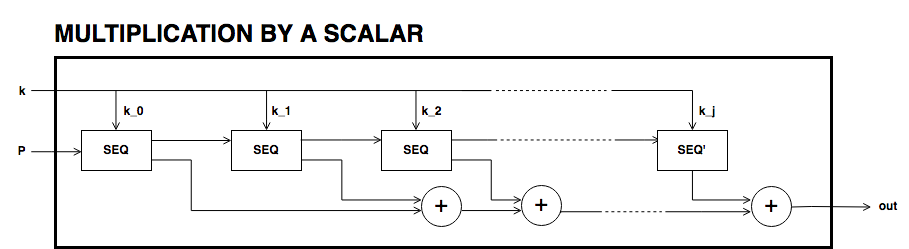
\includegraphics[scale=0.45]{../../figures/multiplication.png}
			\end{figure}
			
			\item Each \textsc{seq} box takes a point of $E$ of the from $P_i = 2^{248 i} P$ for $i=0,\dots,j-1$ and outputs two points %of $E$,
			$$ 	
			2^{248} \cdot P_i 
			\quad \text{and} \quad
			\sum_{n = 0}^{247} b_n \cdot 2^{n} \cdot P_i. 
			$$
			The first point is the input of the next $(i+1)$-th \textsc{seq} box (note that $ 2^{248} \cdot P_i = P_{i+1}$) whereas the second output is the computation of the $i$-th term in expression (\ref{kP}). The precise circuit is depicted in next two figures \textsc{seq} and \textsc{window}.
			
			\begin{figure}[h]
				\centering
				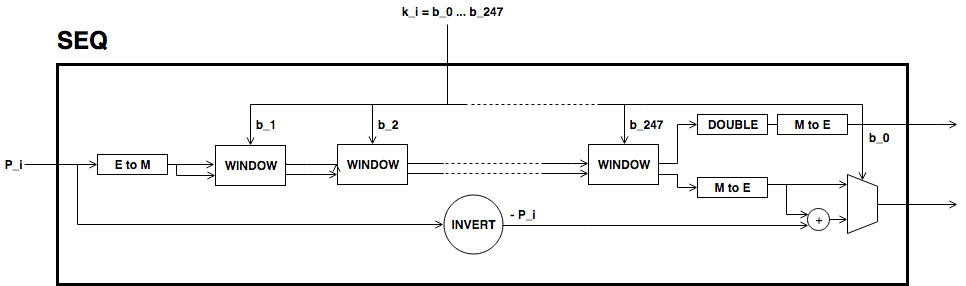
\includegraphics[scale=0.43]{../../figures/multiplication-SEQ.png}\\
				\vspace{0.5cm}
				
				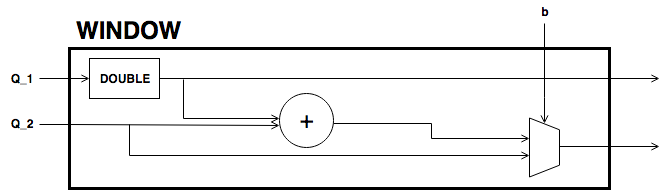
\includegraphics[scale=0.45]{../../figures/multiplication-SEQ-window.png}
				\vspace{0.3cm}
			\end{figure}
			
			The idea of the circuit is to first compute %some point 		
			$$	Q = P_i + b_1 \cdot (2P_i) + b_2 \cdot (4P_i) 
			+ b_3 \cdot (8P_i) + \dots + b_{247} \cdot (2^{247}P_i), $$
			and output the point
			$$ Q - b_0 \cdot P_i. $$
			This permits the computation of $Q$ using the Montgomery form of Baby-Jubjub and only use twisted Edwards for the second calculation. The reason to change forms is that, in the calculation of the output, we may get a sum with input the point at infinity if $b_0 = 0$. 
			
			Still, we have to ensure that none of the points being doubled or added when working in $E_M$ is the point at infinity and that we never add the same two points. 
			
			\begin{itemize}
				
				% None of the points being doubled is the point at infinity.
				\item By assumption, $P\not= O$ and ord$(P)>8$. Hence, by Lagrange theorem {\cite[Corollary 4.12]{lagrange}}, $P$ must have order $r$, $2r$, $4r$ or $8r$. 
				For this reason, none of the points in $E_M$ being doubled or added in the circuit is the point at infinity, because for any integer $m$,  $2^m$ is never a multiple of $r$, even when $2^m$ is larger than $r$, as $r$ is a prime number. Hence, $2^m \cdot P \not= O$ for any $m\in\Z$.		
				
				% Addition: different points.
				\item Looking closely at the two inputs of the sum, it is easy to realize that they have different parity, one is an even multiple of $P_i$ and the other an odd multiple of $P_i$, so they must be different points. Hence, the sum in $E_M$ is done correctly.
			\end{itemize}
			
			\item The last term of expression (\ref{kP}) is computed in a very similar manner. The difference is that the number of bits composing $k_j$ may be shorter and that there is no need to compute $P_{j+1}$, as there is no other \textsc{seq} box after this one. So, there is only output, the point $k_j \cdot P_j = k_j\cdot 2^{248j} P$. This circuit is named \textsc{seq'}.
			
			\begin{figure}[h]
				\centering
				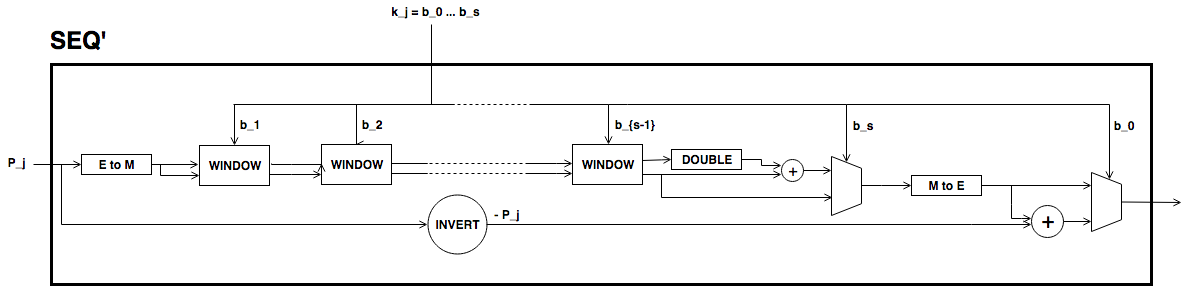
\includegraphics[scale=0.43]{../../figures/multiplication-SEQ-prime.png}
			\end{figure}
			
		\end{enumerate}
		

	\subsection{MiMC-7} \label{sec-mimc}
		
	The specifications we use in the hash are ({\it we are working in explaining this section in greater detail}):
		
	\begin{enumerate}
		\item Number of rounds: $ r = \ceil*{\frac{\llog l}{\llog 7}} = 91. $
		
		\item Inputs: 
				\begin{itemize}
					\item Coordinates of the public key: ($A_x, A_y$).
					\item Coordinates of the point $8R$: ($R8_x, R8_y$).
					\item Message $M$. 
				\end{itemize}
		\item Number of inputs: 5.
		
		\item Generation of constants:  \url{https://github.com/iden3/circomlib/blob/master/src/mimc7.js}.
	\end{enumerate}
		
	\subsection{Example and Test Vectors}
	
	{\it Work in progress.}
	
	\subsection{Existing Implementations}
	
	EdDSA for Baby Jubjub implemented by Jordi Baylina in circom (zero knowledge circuit compiler):\\ \url{https://github.com/iden3/circomlib/blob/master/circuits/eddsamimc.circom}

\section {Intellectual Property}
%	We aim to ensure that proposals can be freely implemented. Thus, proposals should disclose the existence of any known patents (awarded or pending) which may restrict free implementation. This may affect the decision process, and a detailed policy is being developed.

\addcontentsline{toc}{section}{References}
\bibliographystyle{acm}
\bibliography{../../lit}

\end{spacing}
\end{document}
